\documentclass[a4paper,10pt,table]{article}

\usepackage[left=3cm,top=2cm,right=3cm,bottom=3cm,nohead]{geometry} %
\usepackage[utf8]{inputenc}
\usepackage{polski}
\usepackage{pbox}
\usepackage[table,xcdraw]{xcolor}

\usepackage{multirow}

\usepackage{tabularx}

\usepackage{amsmath}
\usepackage{pdfpages}
\usepackage{hyperref}

\usepackage{pgfplots}

\usepackage{placeins}

\usepackage{pgf}

\usepackage{tikz}
\usepackage{caption}
\usepackage{subfigure}
\usepackage{multicol}
\usepackage{xcolor}
\usepackage{listings}
\usepackage{amssymb}


\newtheorem{twr}{Twierdzenie}

\lstdefinestyle{BashInputStyle}{
  language=bash,
  basicstyle=\small\sffamily,
  numbers=left,
  numberstyle=\tiny,
  numbersep=3pt,
  frame=tb,
  columns=fullflexible,
  backgroundcolor=\color{gray!20},
  linewidth=0.9\linewidth,
  xleftmargin=0.1\linewidth
}

\makeatletter
\newcommand{\lstuppercase}{\uppercase\expandafter{\expandafter\lst@token
                           \expandafter{\the\lst@token}}}
\newcommand{\lstlowercase}{\lowercase\expandafter{\expandafter\lst@token
                           \expandafter{\the\lst@token}}}
\makeatother

\lstdefinestyle{Oracle}{basicstyle=\ttfamily,
                        keywordstyle=\lstuppercase,
                        emphstyle=\itshape,
                        showstringspaces=false,
                        }
\lstdefinelanguage[Oracle]{SQL}[]{SQL}{
  morekeywords={ACCESS, MOD, NLS_DATE_FORMAT, NVL, REPLACE, SYSDATE,
                TO_CHAR, TO_NUMBER, TRUNC},
}
\definecolor{light-gray}{gray}{0.95}

\lstset{
  breaklines=true,                                     % line wrapping on
  language=SQL,
  frame=ltrb,
  framesep=5pt,
  basicstyle=\normalsize,
  keywordstyle=\ttfamily\color{green},
  identifierstyle=\ttfamily\color{blue}\bfseries,
  commentstyle=\color{Brown},
  stringstyle=\ttfamily,
  showstringspaces=ture,
  backgroundcolor=\color{light-gray},
  numbers=left
  }



\begin{document}
% \renewcommand{\arraystretch}{1.8}
% \renewcommand{\arraystretch}{1.8}

\begin{titlepage}

\newcommand{\HRule}{\rule{\linewidth}{0.5mm}} % Defines a new command for the horizontal lines, change thickness here

\center % Center everything on the page
 
%----------------------------------------------------------------------------------------
%	HEADING SECTIONS
%----------------------------------------------------------------------------------------

\begin{center}
\includegraphics[scale=0.6]{agh}\end{center}
\vspace*{10mm}
\textsc{\LARGE Akademia Górniczo-Hutnicza}\\[1.5cm] % Name of your university/college
\textsc{\Large Wydział Fizyki i Informatyki Stosowanej}\\[0.5cm] % Major heading such as course name
\textsc{\large Bazy Danych}\\[0.5cm] % Minor heading such as course title

%----------------------------------------------------------------------------------------
%	TITLE SECTION
%----------------------------------------------------------------------------------------

\HRule \\[0.4cm]
{ \huge \bfseries Twarzoksiążka - Portal Społecznościowy
}\\[0.4cm] % Title of your document
\HRule \\[1.5cm]
 
%----------------------------------------------------------------------------------------
%	AUTHOR SECTION
%----------------------------------------------------------------------------------------

\begin{minipage}{0.4\textwidth}
\begin{flushleft} \large
\emph{Autor:}\\
Maciej Kubicki\\
\end{flushleft}
\end{minipage}
~
\begin{minipage}{0.4\textwidth}
\begin{flushright} \large
\emph{Prowadzący:} \\
dr inż. Mirosław Zimnoch
\end{flushright}
\end{minipage}\\[4cm]

% If you don't want a supervisor, uncomment the two lines below and remove the section above
%\Large \emph{Author:}\\
%John \textsc{Smith}\\[3cm] % Your name

%----------------------------------------------------------------------------------------
%	DATE SECTION
%----------------------------------------------------------------------------------------

{\large \today}\\[3cm] % Date, change the \today to a set date if you want to be precise

%----------------------------------------------------------------------------------------
%	LOGO SECTION
%----------------------------------------------------------------------------------------

%\includegraphics{Logo}\\[1cm] % Include a department/university logo - this will require the graphicx package
 
%----------------------------------------------------------------------------------------

\vfill % Fill the rest of the page with whitespace


\end{titlepage}
\newpage
\tableofcontents
\newpage
%------------------------------1-------------------------------
\section{Wstęp teoretyczny}
\subsection{Koncepcja projektu}
Celem projektu jest stworzenie bazy danych realizującej podstawowe wymagania portalu społecznościowego oraz opracowanie wygodnego i przejrzystego interfejsu dla użytkowników. Baza danych wykonana zostanie w systemie PostgreSQL, a aplikacja ją obsługująca przy pomocy technologi PHP, HTML, JavaScript, AJAX, CSS.
\subsection{Analiza wymagań}
Podstawowe wymagania jakie projekt musi spełniać zostały ustalone na podstawie analizy szeroko dostępnych portali społecznościowych, takich jak Facebook, Google+ oraz kilku innych. Podstawowa funkcjonalność obejmuje prezentacje danych użytkownika, możliwość aktualizacji tych danych, system gromadzenia znajomych, system blokowania użytkowników i różnego rodzaju wymiana informacji między użytkownikami portalu:
\begin{itemize}
\item System tworzenia konwersacji i wysyłania wiadomości,
\item System statusów,
\end{itemize}
Kolejną ważną funkcjonalnością jest system dodawania i przeglądania zdjęć. Nie mniej ważna jest opcja wyszukiwania użytkowników. Dodatkowo ciekawa jest funkcjonalność oceny profili użytkowników.
\newpage
\section{Projekt diagramów}
\subsection{Diagram przypływu danych}
Diagram przepływu danych (ang. DFD - data flow diagram) pokazuje w jaki sposób przepływają informacje między procesami oraz bazą. Procesy są wywoływane przez konkretnych aktorów. W moim projekcie wyróżniłem dwóch aktorów:
\begin{itemize}
\item Użytkownik zalogowany,
\item Użytkownik niezalogowany.
\end{itemize}
Każdy aktor ma dostęp do konkretnych procesów. Wykonywany proces zwykle potrzebuje danych od aktora, bądź też z bazy danych. Proces zwraca jakieś dane do aktora, do bazy, bądź też wywołuje kolejny proces.

\begin{figure}[h]
\begin{center}
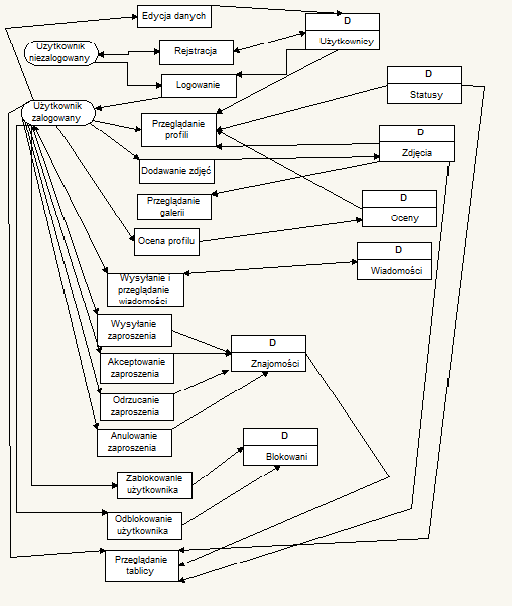
\includegraphics[scale=0.9]{dfd}
\caption{Diagram DFD}
\end{center}
\end{figure}
\newpage
\subsection{Diagram ERD}
Diagram związków encji (ang. Entity-Relationship Diagram) - rodzaj graficznego przedstawienia związków pomiędzy encjami używany w projektowaniu systemów informacyjnych do przedstawienia konceptualnych modeli danych używanych w systemie.
\begin{figure}[h]
\begin{center}
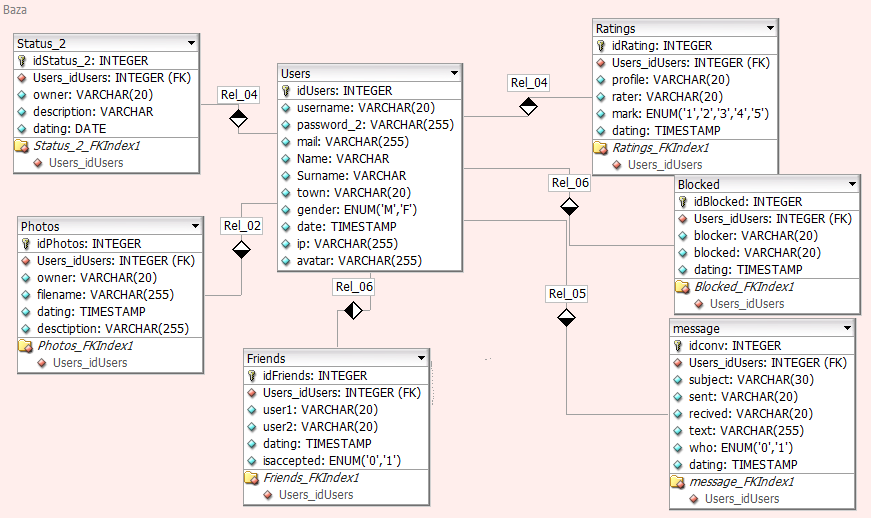
\includegraphics[scale=0.7]{erd}
\caption{Diagram ERD}
\end{center}
\end{figure}
\section{Projekt logiczny}
\subsection{Projekt bazy}
\begin{lstlisting}
           
           
CREATE TYPE Gender AS ENUM('M','F'); 
CREATE TYPE rating AS ENUM('1','2','3','4','5');
CREATE TYPE INVITATION AS ENUM('0','1');
CREATE TYPE owner AS ENUM('0','1');

CREATE TABLE Users (
  idUsers SERIAL   NOT NULL ,
  username VARCHAR(20)   NOT NULL ,
  password VARCHAR(255)   NOT NULL ,
  mail VARCHAR(255)   NOT NULL ,
  Name VARCHAR   NOT NULL ,
  Surname VARCHAR   NOT NULL ,
  town VARCHAR(20)   NOT NULL ,
  gender Gender   NOT NULL ,
  country VARCHAR(255) NOT NULL,
  date timestamp   NOT NULL ,
  ip VARCHAR(255)   NOT NULL,
  avatar VARCHAR(255) NULL,
PRIMARY KEY(idUsers));


CREATE TABLE Photos (
  idPhotos SERIAL   NOT NULL ,
  owner VARCHAR(20)   NOT NULL ,
  filename VARCHAR(255),
  dating timestamp,
  description VARCHAR(255),
PRIMARY KEY(idPhotos));

CREATE TABLE Status (
  idStatus SERIAL   NOT NULL ,
  owner VARCHAR(20)  NOT NULL ,
  description VARCHAR   NOT NULL ,
  dating timestamp   NOT NULL,
PRIMARY KEY(idStatus));

CREATE TABLE Friends (
  idFriends SERIAL   NOT NULL ,
  user1 varchar(20)  NOT NULL ,
  user2 varchar (20) NOT NULL ,
  dating timestamp  NOT NULL ,
  isaccepted INVITATION DEFAULT '0' NOT NULL,
PRIMARY KEY(idFriends));

CREATE TABLE Blocked (
  idblock SERIAL   NOT NULL ,
  blocker varchar(20)  NOT NULL ,
  blocked varchar (20) NOT NULL ,
  dating timestamp   NOT NULL ,
PRIMARY KEY(idblock));

CREATE TABLE message (
	idconv SERIAL NOT NULL,
	subject varchar(30) NOT NULL,
	sent varchar(20) NOT NULL,
	recived varchar(20) NOT NULL,
	text varchar(255) NOT NULL,
	who owner DEFAULT '0',
	dating timestamp NOT NULL,
PRIMARY KEY (idconv));

CREATE TABLE ratings (
	idrating SERIAL NOT NULL,
	profile varchar(20) NOT NULL,
	rater varchar(20) NOT NULL,
	mark rating NOT NULL,
	dating timestamp NOT NULL,
PRIMARY KEY (idrating));




\end{lstlisting}
\begin{itemize}
\item \textbf{Typ gender} - przechowuje płeć,
\item \textbf{Typ rating} - przechowuje możliwe oceny,
\item \textbf{Typ invitation} - przechowuje informacje czy zaproszenie do przyjaźni jest zaakceptowane,
\item \textbf{Typ owner} - przechowuje informacje czy autor konwersacje jest autorem danej wiadomości,
\item \textbf{Tabela users} - zawiera podstawowe informacje o użytkownikach,
\item \textbf{Tabela photos} - zawiera zdjęcia użytkowników,
\item \textbf{Tabela status} - zawiera statusy użytkowników,
\item \textbf{Tabela friends} - zawiera stan znajomości między użytkownikami, gdy wysłane jest zaproszenie do tabeli dodany jest wpis user1 - zapraszający, user2 - zaproszony, isaccepted - czy zaproszenie zostało zaakceptowane,
\item \textbf{Tabela blocked} - zawiera informacje o blokowanych użytkownikach, blocker - osoba blokująca, blocked - osoba zablokowana,
\item \textbf{Tabela message} - zawiera wiadomości wysyłane między użytkownikami, sent - osoba inicjująca konwersacje, recived - uczestnik konwersacji, who - zawiera informacje czy autorem wiadomości jest osoba inicjująca konwersacje,
\item \textbf{Tabela ratings} - zawiera wszystkie oceny profili użytkowników.
\end{itemize}
\section{Projekt funkcjonalny}
Portal społecznościowy jest dużą aplikacją, zbudowaną z wielu interfejsów. Dane do bazy dodawane, bądź zmieniane są na różne sposoby, między innymi poprzez formularze i przyciski. W zależności od danych w bazie podstrony wyświetlają konkretne rzeczy. W aplikacji będą potrzebne następujące interfejsy:
\begin{itemize}
\item właściciela profilu,
\item profil użytkownika,
\item edycji podstawowych danych,
\item dodawania zdjęć,
\item "tablica", gdzie użytkownik może dodać status i widzi statusy, zdjęcia swoje i wszystkich znajomych,
\item galeria użytkownika,
\item wyszukiwarka,
\item lista znajomych,
\item lista zaproszeń,
\item skrzynka wiadomości,
\item interfejs zmiany zdjęcia profilowego.
\end{itemize}
Kolejnym ważnym elementem w takiej aplikacji jest nawigacja po niej. Ważne, żeby była czytelna dla użytkowników i logiczna.
\newpage
\section{Dokumentacja}
Projekt jest umieszczony na serwerze pascal. Zarówno baza danych, jak i aplikacja. Można się z nią połączyć z sieci wydziałowej, bądź też ustawiając odpowiednie proxy w przeglądarce przy otwartym tunelu do sieci wydziałowej. Link:
\begin{center}
\href{http://pascal.fis.agh.edu.pl/~3kubicki/root/index.php}{\color{blue}{Twarzoksiążka Homepage}}
\end{center}

\begin{figure}[h]
\begin{center}
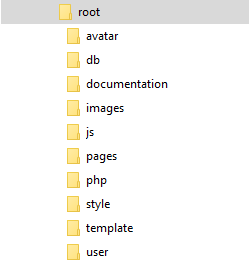
\includegraphics[scale=1]{folder}
\caption{Struktura projektu}
\end{center}
\end{figure}
W katalogu root znajduje się strona startowa \textbf{index.php}.
\begin{itemize}
\item \textbf{avatar} - katalog z avatarami użytkowników, oraz z dwoma domyślnie ustawianymi, jeden dla mężczyzny drugi dla kobiety,
\item \textbf{db} - katalog zawierający skrypt tworzący, kasujący oraz łączący się z bazą,
\item \textbf{documentation} - katalog z dokumentacją,
\item \textbf{images} - wszystkie zdjęcia użyte na podstronach, poza tymi w galerii użytkowników,
\item \textbf{js} - skrypty Javascript,
\item \textbf{pages} - podstrony,
\item \textbf{style} - pliki css,
\item \textbf{php} - skrypty php,
\item \textbf{template} - szablony,
\item \textbf{user} - katalog zawierający podkatalogi użytkowników wraz z ich zdjęciami.
\end{itemize}

\begin{center}
\begin{figure}[h]
\begin{tabular}{|c|c|} 

\hline
\textbf{Username} & \textbf{Password} \\ \hline
harry & harry1 \\ \hline
user & user \\ \hline
maciek94 & trudnehaslo \\ \hline



\end{tabular}
\caption{Przykładowe konta}
\end{figure}
\end{center}
\newpage
\subsection{Użytkowanie aplikacji}
\begin{figure}[h]
\begin{center}
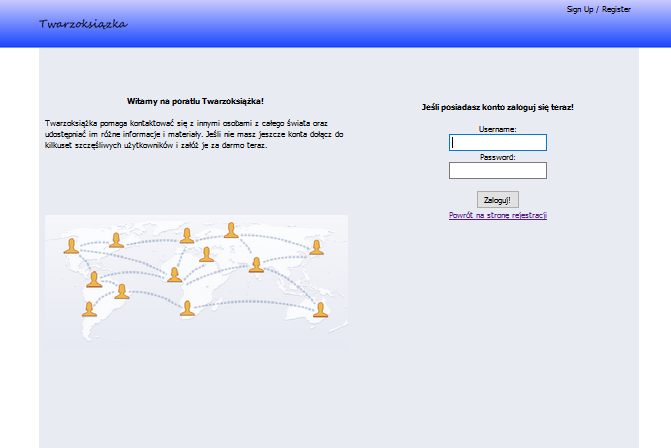
\includegraphics[scale=0.6]{scrn/1}
\end{center}
\end{figure}

Strona główna z formularzem do logowania oraz z odnośnikami do strony rejstracyjnej. Po zalogowaniu jest tworzona sesja. 

\begin{figure}[h]
\begin{center}
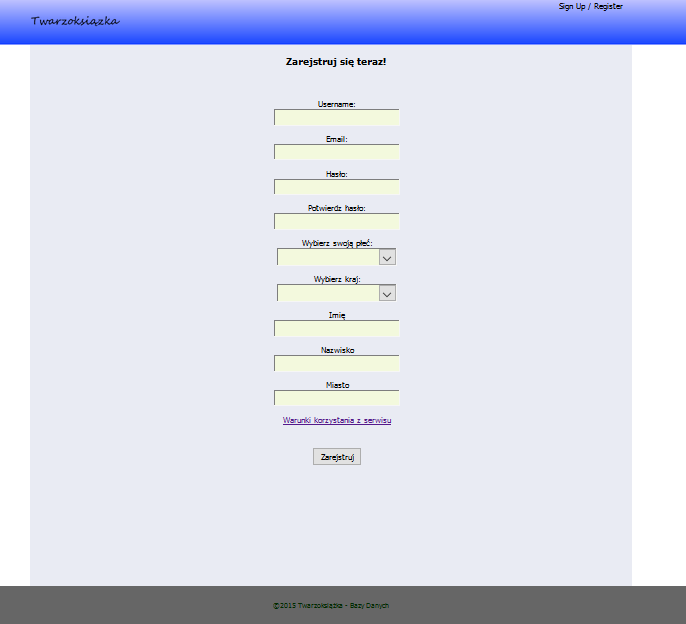
\includegraphics[scale=0.6]{scrn/2}
\end{center}
\end{figure}

Strona rejstracyjna. Dane w formularzu są walidowane po wciśnięciu \textbf{Zarejstruj}. Dodatkowo wcześniej po wpisaniu nazwy użytkownika jest walidowana na bieżąco przy pomocy AJAX. Musi mięć między 3-20 znaków oraz nie może powtórzyć się w bazie. Po wpisaniu nazwy użytkownika na boku pojawia się czy nazwa jest w porządku. Pozostałe dane są walidowane przy pomocy javascriptu oraz AJAX. Mail również nie może się powtórzyć w bazie.
\newpage
\begin{figure}[h]
\begin{center}
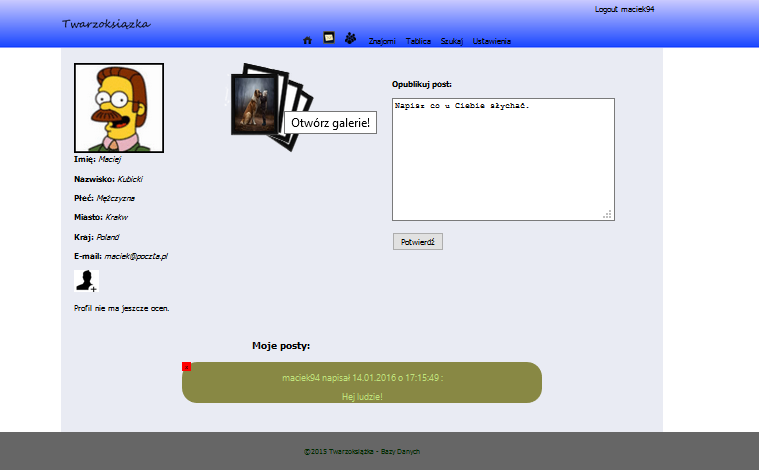
\includegraphics[scale=0.6]{scrn/3}
\end{center}
\end{figure}
Po zalogowaniu otwiera się strona profilowa użytkownika. Na górze mamy menu nawigacyjne. Domek nawiguje do strony profilowej. Koperta do skrzynki wiadomości. Ikonka ludzi do listy zaproszeń wysłanych i odebranych. Jeśli mamy jakieś odebrane zaproszenie to pojawia się tam wykrzyknik. Następne nawigatory są oczywiste: Znajomi - lista znajomych, Tablica - statusy i zdjęcia znajomych, można tam też dodać status, Szukaj - wyszukiwarka znajomych, Ustawienia - ustawienia konta, możliwość zmiany avataru, odblokowania zablokowanych, oraz przycisk wylogowania. Niżej widzimy zdjęcie profilowe, po kliknięciu na nie możemy je zmienić, na prawo widzimy zdjęcie ramek na, na które wrzucamy losowe zdjęcie z galerii, formularz dodanie statusu. Niżej widzimy dane użytkownika, przycisk dodanie zdjęcia, ocene profilu, oraz posty użytkownika, które możemy tu kasować, również przy pomocy AJAX.
\begin{figure}[h]
\begin{center}
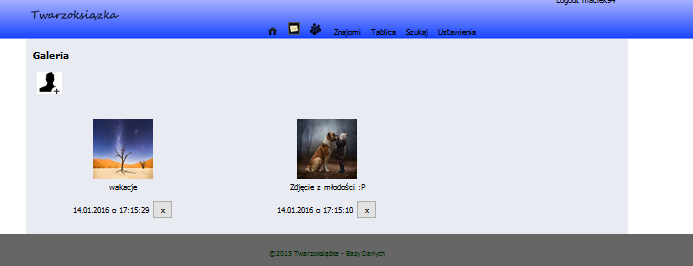
\includegraphics[scale=0.6]{scrn/4}
\end{center}
\end{figure}
Tutaj widzimy galerie własną, jest przycisk dodania zdjęcia oraz kasowania dodanych zdjęć. Po kliknięciu na zdjęcie powiększa się. Aby je zmniejszyć klikamy na nie jeszcze raz. Jeśli wejdziemy do galerii innych użytkowników to nie ma tam przycisków dodania zdjęcia i kasowania zdjęcia.
\newpage
\begin{figure}[h]
\begin{center}
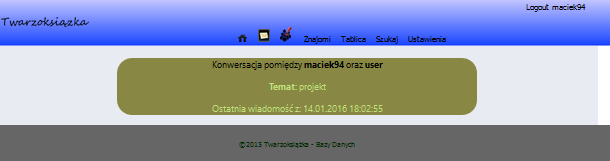
\includegraphics[scale=0.6]{scrn/5}
\end{center}
\end{figure}
Skrzynka odbiorcza z widocznymi otwartymi konwersacjami. Widzimy, że mamy jedną konwersacje, widzimy temat i datę ostatniej wiadomości. Po kliknięciu na konwersacje otwiera się ona:
\begin{figure}[h]
\begin{center}
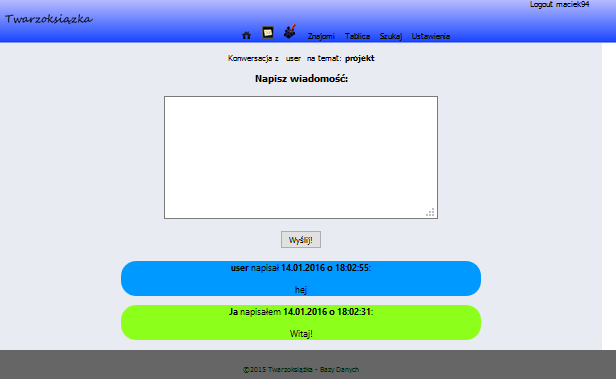
\includegraphics[scale=0.6]{scrn/5b}
\end{center}
\end{figure}\newline
Teraz widzimy wszystkie wiadomości w konwersacji, możemy też dodać wiadomość. Wiadomości "moje" są zielone, a otrzymane błękitne.

\begin{figure}[h]
\begin{center}
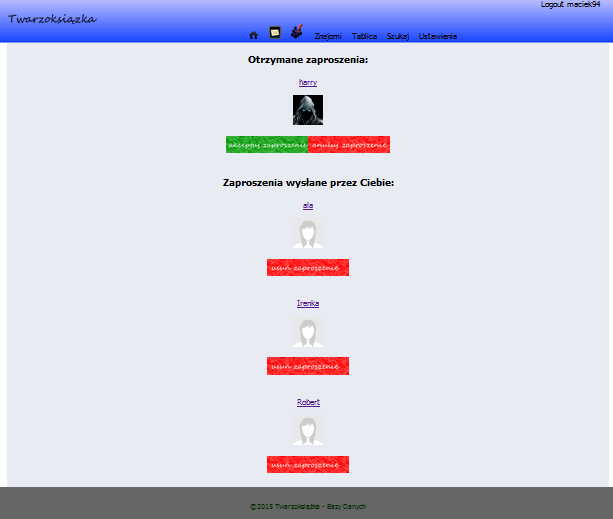
\includegraphics[scale=0.5]{scrn/6}
\end{center}
\end{figure}
Otrzymałem zaproszenie (wykrzyknik się pojawił na ikonce ludzików). Widzimy listę zaproszeń otrzymanych i wysłanych. Możemy przyjąć otrzymane zaproszenie lub nie, a także możemy anulować wysłane zaproszenia.
\newpage
\begin{figure}[h]
\begin{center}
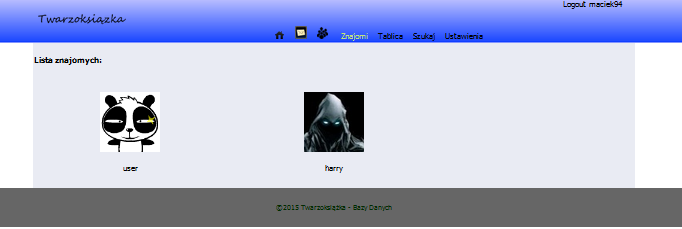
\includegraphics[scale=0.6]{scrn/7}
\end{center}
\end{figure}
Po zaakceptowaniu zaproszenia przechodzę do listy znajomych. Widzę wszystkich moich znajomych. Jest ich dwóch. Klikając na avatar przechodzimy do profilu danego użytkownika.
\begin{figure}[h]
\begin{center}
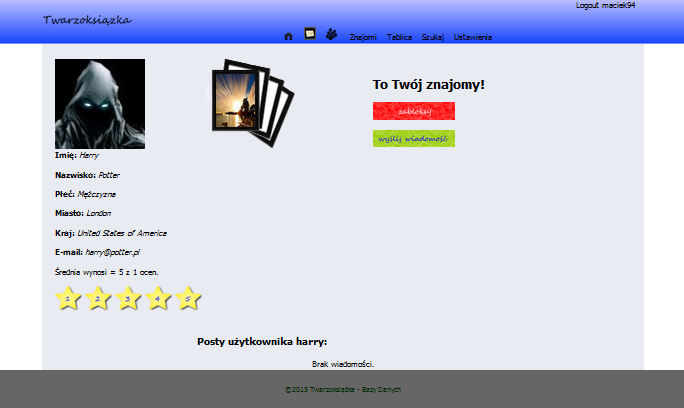
\includegraphics[scale=0.6]{scrn/8}
\end{center}
\end{figure}\newline
Profil innych użytkowników jest bardzo podobny do naszego profilu. Nie ma tu opcji dodawania postu, dodania zdjęć, zmiany avataru. Widzimy tu dane, avatar, ramki ze zdjęciem z galerii użytkownika na którego profilu jesteśmy. Widzimy ocenę jego profilu, jeśli jeszcze nie oceniliśmy go to możemy go ocenić. Widzimy jego posty. Widzimy napis, że to nasz znajomy. Gdyby to nie był nasz znajomy to moglibyśmy wysłać zaproszenie. Dalej widzimy przyciski wyślij wiadomość - otwiera formularzy do wysłania wiadomości o zadanym temacie, jeśli wyślemy do tego użytkownika wiadomość o temacie, który już istnieje między nami to wiadomość zostanie dodana do tamtej konwersacji, jeśli nie to zostanie utworzona nowa konwersacja. Drugi przycisk zablokuj, blokuje wyświetlanie naszego profilu dla tego użytkownika.
\newpage
\begin{figure}[h]
\begin{center}
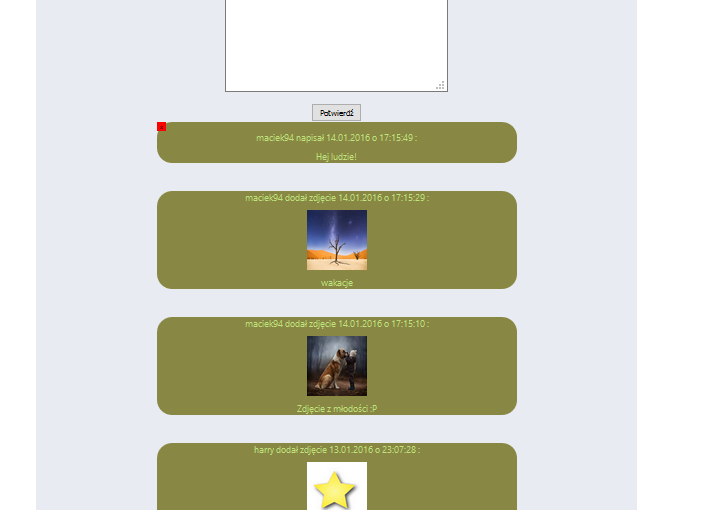
\includegraphics[scale=0.5]{scrn/9}
\end{center}
\end{figure}
Przechodząc na tablice widzimy wszystkie nasze i znajomych statusy i zdjęcia. Możemy też dodać tu status i skasować nasze statusy.
\begin{figure}[h]
\begin{center}
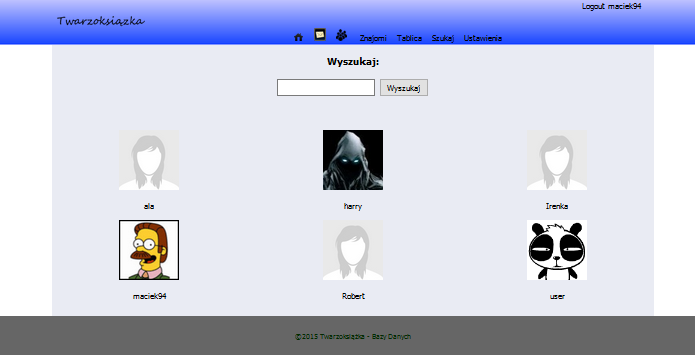
\includegraphics[scale=0.5]{scrn/10}
\end{center}
\end{figure}\newline
Przechodząc do wyszukiwarki mamy możliwość wyszukania znajomych. Nie wpisując żadnego klucza wyszukiwania i wciskając wyszukaj znajdziemy wszystkich użytkowników posortowanych alfabetycznie według nazwy użytkownika.
\begin{figure}[h]
\begin{center}
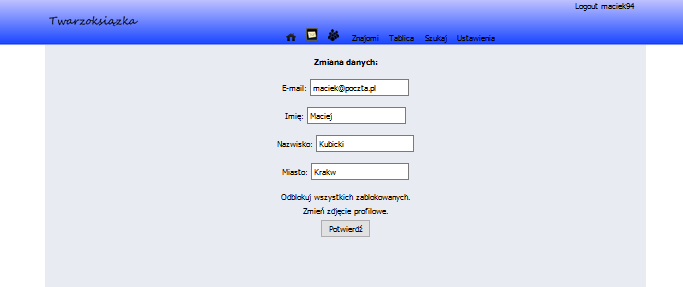
\includegraphics[scale=0.65]{scrn/11}
\end{center}
\end{figure}\newline
Oto panel zmiany ustawień.
\newpage
\begin{figure}[h]
\begin{center}
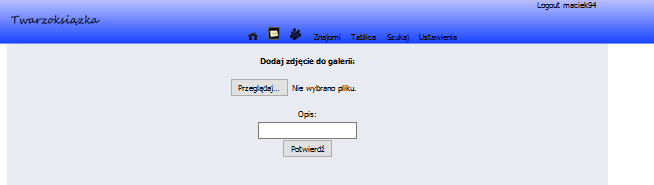
\includegraphics[scale=0.65]{scrn/12}
\end{center}
\end{figure}
Oto formularz dodania zdjęcia.
\begin{figure}[h]
\begin{center}
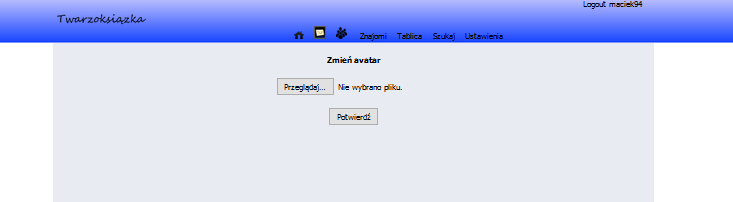
\includegraphics[scale=0.65]{scrn/14}
\end{center}
\end{figure}\newline
Oto formularz zmiany awataru.
\subsection{Możliwości rozwoju}
Projekt pozostawia szerokie możliwości dalszego rozwoju. Przede wszystkim przydałby się panel administratora, który mógłby zarządzać bazą. Mógłby wysyłać jakieś ostrzeżenia do użytkowników, kasować nieaktywne konta. Dla użytkowników dodałoby się prawo zgłoszenia naruszenia regulaminu przez innych użytkowników i administrator mógłby się tym zająć.
Patrząc z drugiej strony jakiś system wydarzeń byłby dobrym pomysłem. Możliwość stworzenie wydarzenia oraz zaproszenie konkretnych użytkowników.
Kolejnym pomysłem jest rozwój galerii użytkowników, którzy mogliby tworzyć podgalerię i dodawać do nich zdjęcia.
Można by dodać system aktywacji konta po otrzymaniu maila oraz przypominania hasła.
Tak więc istnieje wiele dróg rozwoju.


\end{document}

